%  A simple AAU PhD thesis template (collection of papers).
%  2013-05-26 v. 1.1.0
%  Copyright 2012-2013 by Jesper Kjær Nielsen <jkn@es.aau.dk>
%
%  This is free software: you can redistribute it and/or modify
%  it under the terms of the GNU General Public License as published by
%  the Free Software Foundation, either version 3 of the License, or
%  (at your option) any later version.
%
%  This is distributed in the hope that it will be useful,
%  but WITHOUT ANY WARRANTY; without even the implied warranty of
%  MERCHANTABILITY or FITNESS FOR A PARTICULAR PURPOSE.  See the
%  GNU General Public License for more details.
%
%  You can find the GNU General Public License at <http://www.gnu.org/licenses/>.
%
%  A simple AAU PhD thesis template (collection of papers).
%  2013-05-26 v. 1.1.0
%  Copyright 2012-2013 by Jesper Kjær Nielsen <jkn@es.aau.dk>
%
%  This is free software: you can redistribute it and/or modify
%  it under the terms of the GNU General Public License as published by
%  the Free Software Foundation, either version 3 of the License, or
%  (at your option) any later version.
%
%  This is distributed in the hope that it will be useful,
%  but WITHOUT ANY WARRANTY; without even the implied warranty of
%  MERCHANTABILITY or FITNESS FOR A PARTICULAR PURPOSE.  See the
%  GNU General Public License for more details.
%
%  You can find the GNU General Public License at <http://www.gnu.org/licenses/>.
%
\documentclass[10pt,oneside,b5paper,openright]{book}
%%%%%%%%%%%%%%%%%%%%%%%%%%%%%%%%%%%%%%%%%%%%%%%%
% Language, Encoding and Fonts
% http://en.wikibooks.org/wiki/LaTeX/Internationalization
%%%%%%%%%%%%%%%%%%%%%%%%%%%%%%%%%%%%%%%%%%%%%%%%
% Select encoding of your inputs. Depends on
% your operating system and its default input
% encoding. Typically, you should use
%   Linux  : utf8 (most modern Linux distributions)
%            latin1 
%   Windows: ansinew
%            latin1 (works in most cases)
%   Mac    : applemac
% Notice that you can manually change the input
% encoding of your files by selecting "save as"
% an select the desired input encoding. 
\usepackage[utf8]{inputenc}
% Make latex understand and use the typographic
% rules of the language used in the document.
\usepackage[danish,english]{babel}
% Use the vector font Latin Modern which is going
% to be the default font in latex in the future.
\usepackage{lmodern}
% Choose the font encoding
\usepackage[T1]{fontenc}
%%%%%%%%%%%%%%%%%%%%%%%%%%%%%%%%%%%%%%%%%%%%%%%%
% Graphics and Tables
% http://en.wikibooks.org/wiki/LaTeX/Importing_Graphics
% http://en.wikibooks.org/wiki/LaTeX/Tables
% http://en.wikibooks.org/wiki/LaTeX/Colors
%%%%%%%%%%%%%%%%%%%%%%%%%%%%%%%%%%%%%%%%%%%%%%%%
% load a colour package
\usepackage{xcolor}
\definecolor{aaublue}{RGB}{33,26,82}% dark blue
% The standard graphics inclusion package
\usepackage{graphicx}
% Set up how figure and table captions are displayed
\usepackage{caption}
\captionsetup{%
  font=footnotesize,% set font size to footnotesize
  labelfont=bf % bold label (e.g., Figure 3.2) font
}
% Make the standard latex tables look so much better
\usepackage{array,booktabs}
\usepackage{tabularx}
% Enable the use of frames around, e.g., theorems
% The framed package is used in the example environment
\usepackage{framed}
% Create beautiful plots using TikZ and PGFPLOTS
\usepackage{tikz,pgfplots}
\usetikzlibrary{patterns}
%%% commented by KK (ShareLaTeX team) because of compilation errors
%%%\pgfrealjobname{master} % this line enables us to compile figures separately
%%%%%%%%%%%%%%%%%%%%%%%%%%%%%%%%%%%%%%%%%%%%%%%%
% Mathematics
% http://en.wikibooks.org/wiki/LaTeX/Mathematics
%%%%%%%%%%%%%%%%%%%%%%%%%%%%%%%%%%%%%%%%%%%%%%%%
% Defines new environments such as equation,
% align and split 
\usepackage{amsmath}
% Adds new math symbols
\usepackage{amssymb}
% Use theorems in your document
% The ntheorem package is also used for the example environment
% When using thmmarks, amsmath must be an option as well. Otherwise \eqref doesn't work anymore.
\usepackage[framed,amsmath,amsthm,thmmarks]{ntheorem}

%%%%%%%%%%%%%%%%%%%%%%%%%%%%%%%%%%%%%%%%%%%%%%%%
% Page Layout and appearance
% http://en.wikibooks.org/wiki/LaTeX/Page_Layout
%%%%%%%%%%%%%%%%%%%%%%%%%%%%%%%%%%%%%%%%%%%%%%%%
% Change margins, papersize, etc of the document
\usepackage[
  outer=2.25cm, % right margin on an odd page
  inner=1cm, % left margin on an odd page
  bindingoffset=1cm
  ]{geometry}
% Modify how \chapter, \section, etc. look
\renewcommand{\thesection}{\arabic{section}}
% The titlesec package is very configureable
\usepackage{titlesec}
\titleformat*{\section}{\normalfont\Large\bfseries\color{aaublue}}
\titleformat*{\subsection}{\normalfont\large\bfseries\color{aaublue}}
\titleformat*{\subsubsection}{\normalfont\normalsize\bfseries\color{aaublue}}
%\titleformat*{\paragraph}{\normalfont\normalsize\bfseries\color{aaublue}}
%\titleformat*{\subparagraph}{\normalfont\normalsize\bfseries\color{aaublue}}
% Change some default names
\addto\captionsenglish{%this line is required when using the babel package
  \renewcommand\appendixname{Paper} % change Appendix to Paper
  \renewcommand\bibname{References} % change Bibliography to references
  \renewcommand\figurename{Fig.} % change Figure to Fig.
}

% Change the headers and footers
\usepackage{fancyhdr}
\pagestyle{fancy}
\fancyhf{} %delete everything
\renewcommand{\headrulewidth}{0pt} %remove the horizontal line in the header
\fancyhead[RE]{\color{aaublue}\small\nouppercase\leftmark} %even page - chapter title
\fancyhead[LO]{\color{aaublue}\small\nouppercase\rightmark} %uneven page - section title
\fancyhead[LE,RO]{\thepage} %page number on all pages
% Do not stretch the content of a page. Instead,
% insert white space at the bottom of the page
\raggedbottom
% Enable arithmetics with length. Useful when
% typesetting the layout.
\usepackage{calc}
% Enable conditional statements
\usepackage{ifthen}
\ifthenelse{\equal{\jobname}{\detokenize{master}}}{%
%	\usepackage[cam,info,a4,center]{crop} % do not crop pages when compiling tikz-figures
	\usepackage[a4,center]{crop} % do not crop pages when compiling tikz-figures
}{}

%%%%%%%%%%%%%%%%%%%%%%%%%%%%%%%%%%%%%%%%%%%%%%%%
% Bibliography
% http://en.wikibooks.org/wiki/LaTeX/Bibliography_Management
%%%%%%%%%%%%%%%%%%%%%%%%%%%%%%%%%%%%%%%%%%%%%%%%
% Bibliography for each chapter
\usepackage[sectionbib]{chapterbib}
% Custom bibliograhy - used in the list of papers
%\usepackage{multibib}
%\newcites{main}{Main References}
%\newcites{other}{Other Publications}
% Change [1,2,3,4] into [1-4]
\usepackage{cite}

%%%%%%%%%%%%%%%%%%%%%%%%%%%%%%%%%%%%%%%%%%%%%%%%
% Misc
%%%%%%%%%%%%%%%%%%%%%%%%%%%%%%%%%%%%%%%%%%%%%%%%
% Add bibliography and index to the table of
% contents
\usepackage[nottoc,section]{tocbibind}
% Enable subappendices
\usepackage{appendix}
\renewcommand{\setthesection}{\Alph{section}} % remove the chapter numbering
% Add the command \pageref{LastPage} which refers to the
% page number of the last page
\usepackage{lastpage}
% Add notes to in your document
\usepackage[
%  disable, %turn off todonotes
  colorinlistoftodos, %enable a coloured square in the list of todos
  textwidth=\marginparwidth, %set the width of the todonotes
  textsize=scriptsize, %size of the text in the todonotes
  ]{todonotes}

%%%%%%%%%%%%%%%%%%%%%%%%%%%%%%%%%%%%%%%%%%%%%%%%
% Hyperlinks
% http://en.wikibooks.org/wiki/LaTeX/Hyperlinks
%%%%%%%%%%%%%%%%%%%%%%%%%%%%%%%%%%%%%%%%%%%%%%%%
% Enable hyperlinks and insert info into the pdf
% file. Hypperref should be loaded as one of the 
% last packages
\usepackage{hyperref}
\hypersetup{%
	pdfpagelabels=true,%
	plainpages=false,%
	pdfauthor={Author},%
	pdftitle={Title},%
	pdfsubject={Subject},%
	bookmarksnumbered=true,%
	colorlinks=true,%
	citecolor=aaublue,%
	filecolor=aaublue,%
	linkcolor=aaublue,% you should probably change this to black before printing
	urlcolor=aaublue,%
	pdfstartview=FitH%
}
% package inclusion and set up of the document
% see, e.g., http://en.wikibooks.org/wiki/LaTeX/Formatting#Hyphenation
% for more information on word hyphenation
\hyphenation{ex-am-ple hy-phen-a-tion short}
\hyphenation{long la-tex}
% 
%  A simple AAU PhD thesis template (collection of papers).
%  2013-05-26 v. 1.1.0
%  Copyright 2012-2013 by Jesper Kjær Nielsen <jkn@es.aau.dk>
%
%  This is free software: you can redistribute it and/or modify
%  it under the terms of the GNU General Public License as published by
%  the Free Software Foundation, either version 3 of the License, or
%  (at your option) any later version.
%
%  This is distributed in the hope that it will be useful,
%  but WITHOUT ANY WARRANTY; without even the implied warranty of
%  MERCHANTABILITY or FITNESS FOR A PARTICULAR PURPOSE.  See the
%  GNU General Public License for more details.
%
%  You can find the GNU General Public License at <http://www.gnu.org/licenses/>.
%
%
%
% see, e.g., http://en.wikibooks.org/wiki/LaTeX/Customizing_LaTeX#New_commands
% for more information on how to create macros

%%%%%%%%%%%%%%%%%%%%%%%%%%%%%%%%%%%%%%%%%%%%%%%%
% Environment
%%%%%%%%%%%%%%%%%%%%%%%%%%%%%%%%%%%%%%%%%%%%%%%%
%example
\theoremheaderfont{\normalfont\bfseries}
\theorembodyfont{\normalfont}
\theoremstyle{break}
\def\theoremframecommand{{\color{aaublue!50}\vrule width 5pt \hspace{5pt}}}
\newshadedtheorem{exa}{Example}[section]
\newenvironment{example}[1]{%
		\begin{exa}[#1]
}{%
		\end{exa}
}

%assumptions
\newtheorem{ass}{Assumption}[section] % assumptions

%%%%%%%%%%%%%%%%%%%%%%%%%%%%%%%%%%%%%%%%%%%%%%%%
% Paper Inclusion
%%%%%%%%%%%%%%%%%%%%%%%%%%%%%%%%%%%%%%%%%%%%%%%%
% include a paper
\newcommand{\includepaper}[1]{
  \cleardoublepage
  \setcounter{enumiii}{0}
  \setcounter{enumii}{0}
  \setcounter{enumiv}{0}
  \setcounter{enumi}{0}
  \setcounter{equation}{0}
  \setcounter{figure}{0}
  \setcounter{footnote}{0}
%  \setcounter{lofdepth}{1}
%  \setcounter{lotdepth}{1}
  \setcounter{mpfootnote}{0}
  \setcounter{paragraph}{0}
  \setcounter{parentequation}{0}
  \setcounter{part}{0}
  \setcounter{section}{0}
%  \setcounter{subfigure}{0}
  \setcounter{subparagraph}{0}
  \setcounter{subsection}{0}
  \setcounter{subsubsection}{0}
%  \setcounter{subtable}{0}
  \setcounter{table}{0}
  \include{#1}
}

% create the paper titlepage
\newcommand{\papertitlepage}[5]{
  \chapter{#1}\label{#2}
  \chaptermark{}
  \vspace{2cm}
  \begin{center}
    \large #3
  \end{center}
  \vspace{3cm}
  \begin{center}
  \normalsize #4
  \end{center}
  \vspace*{\fill}
  \newpage\thispagestyle{empty}
  \vspace*{\fill}
    #5\par
    \noindent{\em The layout has been revised.}
  \vspace*{\fill}
  \cleardoublepage
}

% environment for abstracts
\newenvironment{abstract}{\section*{Abstract}\it}{}


%%%%%%%%%%%%%%%%%%%%%%%%%%%%%%%%%%%%%%%%%%%%%%%%
% Various names
%%%%%%%%%%%%%%%%%%%%%%%%%%%%%%%%%%%%%%%%%%%%%%%%
\newcommand{\IEEEPARstart}[2]{#1#2}


%%%%%%%%%%%%%%%%%%%%%%%%%%%%%%%%%%%%%%%%%%%%%%%%
% Bibliography
%%%%%%%%%%%%%%%%%%%%%%%%%%%%%%%%%%%%%%%%%%%%%%%%
\newcommand{\defaultbib}{%
  \bibliographystyle{IEEEtran}
  \bibliography{bib/mybib}
}

\newcommand{\aautitlepage}[3]{%
  {
    %set up various length
    \ifx\titlepageleftcolumnwidth\undefined
      \newlength{\titlepageleftcolumnwidth}
      \newlength{\titlepagerightcolumnwidth}
    \fi
    \setlength{\titlepageleftcolumnwidth}{0.5\textwidth-\tabcolsep}
    \setlength{\titlepagerightcolumnwidth}{\textwidth-2\tabcolsep-\titlepageleftcolumnwidth}
    %create title page
    \thispagestyle{empty}
    \noindent%
    \begin{tabular}{@{}ll@{}}
      \parbox{\titlepageleftcolumnwidth}{
        \iflanguage{danish}{%
          \includegraphics[width=\titlepageleftcolumnwidth]{figures/aau_logo_da}
        }{%
          
\includegraphics[width=\titlepageleftcolumnwidth]{frontmatter/aau_logo_en.pdf}
        }
      } &
      \parbox{\titlepagerightcolumnwidth}{\raggedleft\sf\small
        #2
      }\bigskip\\
       #1 &
      \parbox[t]{\titlepagerightcolumnwidth}{%
      \textbf{Abstract:}\bigskip\par
        \fbox{\parbox{\titlepagerightcolumnwidth-2\fboxsep-2\fboxrule}{%
          #3
        }}
      }\\
    \end{tabular}
    \vfill
    \iflanguage{danish}{%
      %\noindent{\footnotesize\emph{Rapportens indhold er frit tilgængeligt, men offentliggørelse (med kildeangivelse) må kun ske efter aftale med forfatterne.}}
    %}{%
      %\noindent{\footnotesize\emph{The content of this report is freely available, but publication (with reference) may only be pursued due to agreement with the author.}}
    }
    \clearpage
  }
}

%Create english project info
\newcommand{\englishprojectinfo}[8]{%
  \parbox[t]{\titlepageleftcolumnwidth}{
    \textbf{Title:}\\ #1\bigskip\par
    \textbf{Theme:}\\ #2\bigskip\par
    \textbf{Project Period:}\\ #3\bigskip\par
    \textbf{Project Group:}\\ #4\bigskip\par
    \textbf{Participant(s):}\\ #5\bigskip\par
    \textbf{Supervisor(s):}\\ #6\bigskip\par
    \textbf{Copies:} #7\bigskip\par
    \textbf{Page Numbers:} \pageref{LastPage}\bigskip\par
    \textbf{Date of Completion:}\\ #8
  }
}
% my new macros

\begin{document}
%frontmatter
\frontmatter
\pagestyle{empty} %disable headers and footers
\pagenumbering{roman} %use roman page numbering in the frontmatter
%  A simple AAU PhD thesis template (collection of papers).
%  2013-05-26 v. 1.1.0
%  Copyright 2013 by Jesper Kjær Nielsen <jkn@es.aau.dk>
%
%  This is free software: you can redistribute it and/or modify
%  it under the terms of the GNU General Public License as published by
%  the Free Software Foundation, either version 3 of the License, or
%  (at your option) any later version.
%
%  This is distributed in the hope that it will be useful,
%  but WITHOUT ANY WARRANTY; without even the implied warranty of
%  MERCHANTABILITY or FITNESS FOR A PARTICULAR PURPOSE.  See the
%  GNU General Public License for more details.
%
%  You can find the GNU General Public License at <http://www.gnu.org/licenses/>.
%
\pdfbookmark[0]{Front page}{label:frontpage}%
\begin{titlepage}
  \addtolength{\hoffset}{0.5\evensidemargin-0.5\oddsidemargin} %set equal margins on the frontpage - remove this line if you want default margins
  \noindent%
  \begin{tabular}{@{}p{\textwidth}@{}}
    \toprule[2pt]
    \midrule
    \vspace{0.2cm}
    \begin{center}
    \Huge{\textbf{
      Pick and Place
    }}
    \end{center}
\hspace{2.5cm}
      \makebox[0pt][l]{%
  \raisebox{-\totalheight}[0pt][0pt]{%
    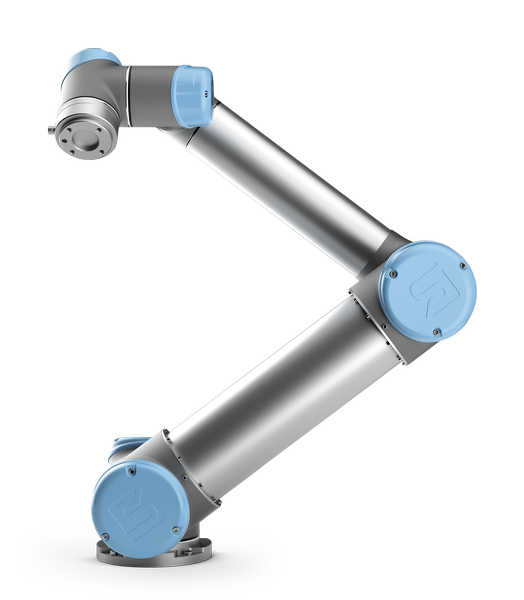
\includegraphics[width=6in]{frontmatter/UR51.png}}}%
    \vspace{0.2cm}\\
    \midrule
    \toprule[2pt]
  \end{tabular}
  \vspace{7 cm}
  \begin{center}
    {\large
      2nd. semester 2018 - ROB2 B229%Insert document type (e.g., Project Report)
    }\\
    \vspace{1cm}
    {\Large
      %Insert your group name or real names here
    }
  \end{center}
  \vfill
  \begin{center}
  Aalborg University\\
  DK-9220 Aalborg
  \end{center}
\end{titlepage}
\clearpage

% mainfile: ../master.tex
\chapter*{Abstract\markboth{Abstract}{Abstract}}\label{ch:Abstract}
\addcontentsline{toc}{chapter}{Abstract}
English abstract



\pdfbookmark[0]{Contents}{label:contents}
\pagestyle{fancy} %enable headers and footers again
\tableofcontents

\chapter*{Preface\markboth{Preface}{Preface}}\label{ch:preface}
\addcontentsline{toc}{chapter}{Preface}


\vspace{\baselineskip}\hfill Aalborg University, \today
\vfill\noindent
\begin{minipage}[b]{0.45\textwidth}
 \centering
 \rule{\textwidth}{0.5pt}\\
  Valdemar Jul Qvist\\
 {\footnotesize <vqvist17@student.auu.dk>}
\end{minipage}
\hfill
\begin{minipage}[b]{0.45\textwidth}
 \centering
 \rule{\textwidth}{0.5pt}\\
  Mark Richard Blankensteiner\\
 {\footnotesize <mblank16@student.aau.dk>}
\end{minipage}
\vspace{3\baselineskip}
\begin{center}
\begin{minipage}[b]{0.45\textwidth}
 \centering
 \rule{\textwidth}{0.5pt}
  Anders Fischer Steen Jensen\\
 {\footnotesize <afsj16@student.aau.dk>}\\
\end{minipage}
\hfill
\begin{minipage}[b]{0.45\textwidth}
 \centering
 \rule{\textwidth}{0.5pt}\\
  Jonathan Midtgaard Jensen\\
 {\footnotesize <jonjen16@student.aau.dk>}
\end{minipage}
\end{center}
\cleardoublepage

%mainmatter
\mainmatter
\chapter{Introduction} \label{ch:introduction}

This project takes the perspective of a research and development team at Grundfos, with the task of creating a work-cell for the production of a rotor, using a flexible workstation. The workstation can be mounted with a manipulator, which can be programmed to perform various tasks within a work cell. The manipulator is meant for use in collaboration with human operators and employees.\\ 
A work-cell has to be designed based upon a number of requirements set in the case description.\\



\section{History of Grundfos} \label{ch:History of Grundfos}

In 1945 Poul Due Jensen founded what later became Grundfos in 1967. He started from his basement, where he did plumbings and blacksmith work, and had two employees\cite{documentray}.\\
\\
Once Poul Due was asked by a local farmer if he could install a motor driven water pump at his farm. He searched for such a pump, but there was none available on market due to the crisis after the second world war. 
He then created his first pump known as "The Pig", which he engineered from scratch, afterwards his production expanded quickly. 
One of Poul's inventions was the Grundfos-carousel. This carousel moves components around two different workstations, some of which are still running 24 hours a day\cite{documentray}.\\
\\
Poul gave Grundfos some founding principles to follow, which were social responsibilities towards employees and the local community.
The business kept expanding, and now there are 19.000 employees, which produce approximately 16 million pumps per year\cite{1Grundfos}.\\
\\
Worth mentioning is one of their core values which the company is built around.\\

   
\paragraph{Sustainability.} Grundfos is following the goals, which are set in the UN sustainability goals, number 6 \cite{Ggoal6}. These goals are meant to lower the water stress level around the world, and to provide clean water efficiently \cite{goal6}.\\
%\item 2. Credibility.\\ This value helps both parts, the buyer and the company. As a big company it is crucial to keep the customers satisfied, and upholding what is promised.\\
%\item 3. Ambitious.\\ At Grundfos they strive to come up with the best solutions without cutting corners.\\
Grundfos is currently using, and further implementing robotic aid to help perform various tasks and streamline the production. With 250 robots and counting, an automated sorting system using robotic manipulators to move parts around, is currently under development and testing. They are a perfect example of how robots are enhancing factory work-flow, and improving the speed and efficiency.  Grundfos is however, already using the KUKA KR30 robot to feed parts directly into machinery, which was previously an expensive and operator intensive process. Among other, these are some of the reasons Grundfos is considered an innovative leading company in their field\cite{1Grundfos},\cite{Grundfosrobot}. 

%\subsection{Factory of the Future}

%Factory of the Future is based on the early stage of the production to shipment and service of the product, linking all the above to fit the customers need.\\
%The red line between the early stages of the pump and the service is based on how many features that is implemented to help the consumers to both save money and use less water. This is the reason Grundfos is the leading company.
%The work-process of the pump is split in to different sections of experts handling the mechanics, hydraulics, marketing etc.\\



\chapter{Case description} \label{ch:case description}

In this project, we are going to focus on the Universal Robot, UR5 which is an industrial manipulator.\\
The UR5 is going to assist in the balancing and leak test of a L40 rotor that is being produced at Grundfos.The L40 rotor is arriving at the work-cell via convoy. The rotor has to go trough a balancing machine, where the rotor is placed in a drawer, after that it has to go through a visual inspection, before it has to be leak tested.\\
The leak testing machine can test two rotors per load, when the leak test is done, the machine will give a signal if the rotor has passed the test or not, if passed it will be placed in an engraving machine that prints the ID of rotor on it, after that it will be place on a pallet, when it is full it will be send a signal to a Grundfos employee to replace the pallet.\\ 
In between the leak machine and the engraving station we can utilize a table as a buffer that has 100 drilled holes for the rotor to be temporarily stored at, furthermore the rotor has to has to go through a cycle in 26 sec or less.

\newpage
\section{Initial problem statement}\label{ch:Initial problem statment}
%How is it possible to give a robotic arm a set of problems to solve, while figuring out the
%coordinate systems of the 3D-space and giving it a set of code to autonomously figure out the algorithm given to it.\\

%This section will identify the initial problems related to the project case given by Grundfos, which will be discussed and examined for this project.

In this project, a work-cell must be created, which can complete the set task of processing pump rotors through 3 different processes and a visual inspection, within a time limit of 26 seconds. The work-cell must be suitable for the collaboration of human employees and robotic manipulators, and be ergonomic for these employees, in order to create a good and safe work environment. \\
To research this the following questions will be answered throughout the problem analysis:

\begin{itemize}

    \item How is it possible to output a balanced, checked, and engraved L40 rotor put in a trolley?
    \item How is it possible to design a work-cell that a manipulator can operate within?
    \item How can each rotor within the work-cell be correctly processed within the required time frame?
    \item  Which legal standards and regulations are required for the safety in the work-cell, and what is required for the cobot to collaborate safely with humans?
\end{itemize}

%\item Which social aspects would impact the employees when implementing the robot?
%\item How is it possible to optimize the UR within the work-cell?
%\item Is the UR manipulator the most suitable for this task?
%\item What is the most efficient design for the end-effector?
%\item How can the robot localize the objects and place the tool correctly?

\chapter{Stakeholder Analysis} \label{ch:Stakeholder Analysis}

\begin{figure}[h]
    \centering
    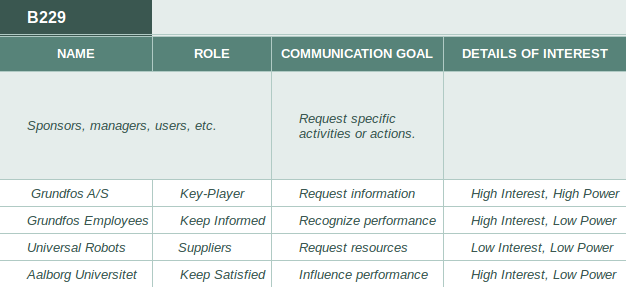
\includegraphics[scale=0.65]{StakeholderAnalysis/Stakeholder.png}
    \caption{Stakeholder Analysis} 
    \label{fig:Stakeholder} 
\end{figure}

\section{Grundfos A/S}\label{ch:grundfosas-stake}
Grundfos A/S is a stakeholder with high interest and high power, as they are investing in the UR. Their interest is high, because the further development of the robotic solution directly impacts the company. Development would be difficult without funding, which also gives Grundfos a lot of power. 


\section{Grundfos Employees}\label{ch:grundfosemp-stake}
Employees of Grundfos are stakeholders, who have a high interest, but a low influence.\\ The reason for this is, that they have no final say in whether the solution should be implemented. The Employees will in some instances have to learn new skills, in order to use the robots.


\section{Universal Robots}\label{ch:Universalrobots-stake}
The suppliers of the robotic manipulator in this case has a low interest and a low power, this is because they do not have any say in the matter. Whether it should be their manipulator or a competitors manipulator, they can then adjust the prices on the manipulator so we would choose their product for this case. 


\section{Aalborg University}\label{ch:Aau-stake}
Aalborg University has an interest in the development of robotics from a research and information perspective. For this reason they potentially have an interest in investing in further development and improvement of a technology such as the UR. 
 \chapter{Technical Analysis} \label{TechAnalysis}
 
 The work cell regarding this project, consists of a number of machines and other articles used in the production of a rotor for one of the pumps at Grundfos. This chapter provides a description of these articles and their function in the work cell.\\
 
 \section{Work-cell}
 
 \subsection{Balancing machine}
 
 The balancing machine is 1.65m in width and 2.0m in length.\\
 The balancing machine is only capable of testing 1 rotor at a time.\\
 The machine consists of 2 rigid pedestals, with bearings and suspension on the top, supporting a mounting platform where the rotor will be placed hanging on the pedestals.\\

The test will function by the machine turning the rotor, while a vibration sensor detects differences of unbalance in the rotor. From that information it can tell where to add or remove weights, to balance the rotor, after which a visual inspection is required.\\

Safety measures might have to be taken, if an employee has to enter the work-space to inspect the rotor.
 
 \subsection{Leak testing machine}
 
 The leak testing machine is 1.2m wide (with control pad), and 1.8m of length.\\ 
 It is used to test the rotors for a leakage, and it can hold up to 2 rotors per test.\\
 Inside the system the rotors are placed in some valves that will tighten around the rotor, and afterwards placed under a certain air pressure, with the valves on the rotor closed. Then the pass/fail decision will be made and the work-cell can continue \cite{LEAK}.\\
 The Machine will then signal the result of the test.\\
 
 The rotors will need to be placed almost simultaneously inside the machine. The Queue table will play a big role of the flow in the work-cell. Installing it closest to the leak-machine will be revised, since the cobot will need to place the newly balanced rotor, and the queued rotor in a matter of seconds.\\ 
 In this motion a safety standard will have to be considered, since the speed and the force of the cobot will be at a high level, and cant be slowed down to get the desired requirement of 26 seconds.\\
 
 \subsection{Laser engraver}
 The engraving machine has a dimension of 0,7m width and 1,3m in length.\\
 It is used to engrave the part number id of rotor, there is space for one rotor per cycle.\\
 The engraver is made with a laser engraver from ROFIN, it uses a set of mirrors to control the laser beam\cite{laser}. The rotor is placed in a fixture inside the engraving machine,then a door that protect people from the harmful laser beam, has to be closed, this can be done from a foot pedal. When the engraving is done the door opens and the rotor can be stored at the pallet.   
 
 \subsection{Queue table}
 The queue table is a box with holes that serves as a temporary storage for the rotors. Up to 100 rotors can be placed here at any given point during the process to rest, and then moved on to the appropriate machine when they are ready. The queue table has a length and width of 51.5 cm. and a height of 80 cm.  
 
 \subsection{Output pallet}
 When the rotors are complete, they can be moved to the output pallet, which can hold up to 320 rotors at a time. When the pallet is full, it will be moved and emptied where the rotors are needed, and then returned by an employee, so it can be filled again. 
 
 \section{Signals}
 
 When the robot needs to operate inside the work-cell it needs to have some systems that will tell it when to pick and place the rotor.\\
 Hereby some candidates are chosen:\\
 1. Lidar\\
 2. Pressure sensors\\
 3. ROS\\
 4. cameras.\\
 
 1. Lidar sensors can be used due to their highly concentrated 3D-point clouds. This will help the cobot to determine the spot for the different activities inside the work-cell.\\
 
 2. Pressure sensors which is included in the cobot, can be used as a weight distributor. Where the cobots payload of the rotor will be released when placed, and then the pressure sensor on the machines, could determine whether it was placed correctly.\\
 \todo{gerne flere forslag til placering rotor}
 
 3. All of the above could be managed with the interface of ROS, where a service program could be included to send messages through the topics of both cobot and machine. Hereby the two collaborating systems could interact between each other and send commands that could be interpreted by the cobot.\\
 
 4.Industrial robots might use extra safety precautions, to decrease the probability of incidents happening. This could be extra sensors detecting when humans enter, or leave their designated workspace. For caged robots, the door to the cage must usually be closed in order for the robot to run, but you might also want other more reactive ways of ensuring the safety of the personal, particularly when using collaborative robots. One of the most used sensors on these kind of robots would be a collision detection sensor. This allows the robot to register when colliding with a soft surface, and the ability to then either stop, or reduce speed.\\

Many other types of safety sensors might be needed when humans are working side by side with robots. This could include cameras, lasers or pressure sensors. Anything that can help letting the robots know, that humans are present.\\

When working in a production, that require the robots to pick up parts, and place them elsewhere, it might be a very good idea to have a part detection sensor. This sensor tells the robot whether it picked something up or not, and potentially if it is picked up in the right way. If something goes wrong, the robot might either send an error message to an operator, or try to repeat the task, depending on the configuration.\\

\section{Possible cobot Solutions} \label{ch:UR}

This section is taking 2 different cobots in to consideration for a possible solution to the case description.

\section{KUKA}

The KUKA company started more than a hundred years ago. They were the first to invent point welding gripper in Germany.\\
As the years goes by the KUKA company writes history by inventing the world first industrial lightweight robot with sensors in every axis.\\

KUKA and Rethink are competitors since they have the same market, hence is why this project will take both in to consideration of a possible optimization of the work-cell\cite{KukaHist}.\\


\subsection{KUKA LBR IIWA 7 R800}
\begin{figure}[h]
    \centering
    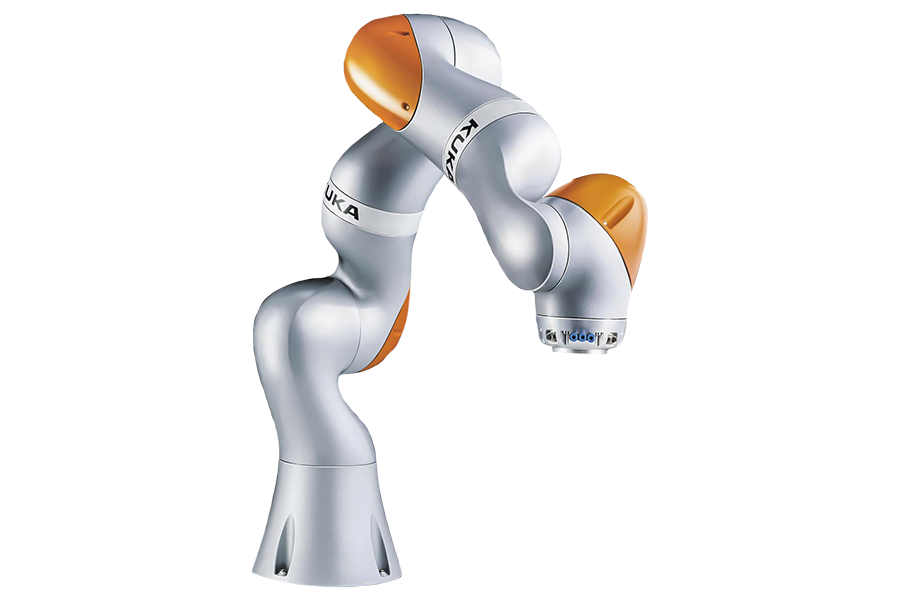
\includegraphics[width=9cm]{UR/1502895088_1.png}
    \caption{KUKA LBR IIWA 7 R800 \cite{KUKAbillede}}
    \label{fig:LBR IIWA}
\end{figure}

Here are the specification for the LBR iiwa 7 R800:\\

\begin{itemize}
    \item Weight: 23.9 kg.
    \item Payload: 7 kg.
    \item Footprint: 136 mm.
    \item Joints: Ranging from +/-120 degrees to +/-170.
    \item Operating life: 30,000 Hours.
    \item Speed: Joints = 180 degrees/sec
    \item Reach: 800-820 mm
    \item Repeatability: +/- 0.1 mm.
\end{itemize}
\cite{KukaSpec1},\cite{KukaSpec2}.

\section{Rethink Robotics}

Rethink robotics was founded in 2000, and are known for their invention the "Roomba Vacuum". They decided to use their knowledge of machinery in the everyday life in factories.\\
The first cobot they designed was in 2012, and was called "Baxter", see \ref{fig:Rethink},\cite{Rethink}.

\subsection{Baxter}
\begin{figure}[h!]
    \centering
    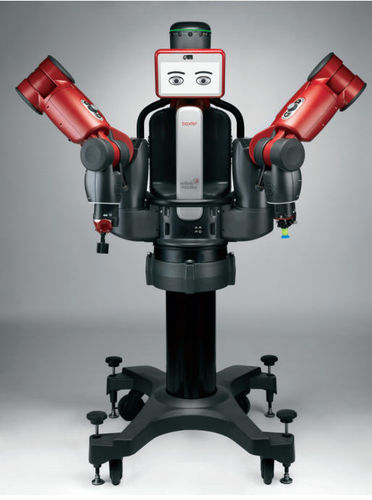
\includegraphics[width=9cm, height=9cm]{UR/baxter-robot-1.jpg}
    \caption{Baxter cobot from "Rethink Robotics"\cite{Rethinkbillede}} 
    \label{fig:Rethink}
\end{figure}

\subsubsection{Specifications for Baxter}
\begin{itemize}
    \item Weight: 75 kg.
    \item Payload: 2.2 kg.
    \item Footprint: 36x32 mm.
    \item Joints: Ranging from +/-175 degrees.
    \item Operating life: ??.
    \item Speed: Joints = 2 to 4 sec per joint rotation.
    \item Reach: 1210 mm
    \item Repeatability: +/- 5 mm.
\end{itemize}
\cite{Rethinkspec}

\subsection{Why cobots?}\label{ch:Whycobot}
Why is there a need for a cobot? A thing that is mentioned in an article about cobots, in an assembly line, is that cobots can help reduce the ergonomics stress level of the employees\cite{Coboau}. Another way this can help the production flow, is that the robot can preform some tedious task while the employee can take care of the complex tasks in the work area.\\

\subsection{Which cobot is more suitable?}

Having the case description in mind \ref{ch:case description}, and the fact that the process must not be more than 26 seconds, before a fully functional rotor is ready.\\
The cobots have almost similar specifications, the only major difference is the rotations of the joints. In this case a huge maneuverability is required, hence the rotation of the joints is a factor weighed highly in this process. Beside that, the only difference would be what would suit the company the most. Since Grundfos has implemented KUKA's is because it is easier to run a production-line with the same system, and the workers know these robots.\\
%The most suitable for this project is UR5.

\subsection{Conclusion}

%Taking all of the above into consideration, some data can be included in the ideal robot for this case.\\ 
%Having an overview of the different tasks that has to be preformed and using the tools that are given, the project can get closer to a conclusion for the robot.\\
%The project has focused on two different cobots, 1 from KUKA, and 1 from UR. They are then set up to conclude which has the better specifications. By looking at nothing else than the specifications, the most suitable for this case is the UR5.\\

\newpage


\chapter{Regulation}\label{ch:regulation}
\subsection{Ergonomic}
According to the Danish labor inspectorate, article 4.05.3 there is a need to consider ergonomic work positions, of the person who has to inspect the rotor.\\
If the person has to do measurements on the rotor, it needs to be in a position where the worker does not have their arms in a stressful position.\\
There is also a need to take into consideration, if it is possible to make the work area more dynamic i.e. sometimes standing or seated this will insure that the person how is inspecting will keep the body function working.\\
There is also the need to make sure the neck and shoulders is not put under stress by looking up or down at the object\cite{ATpostions}.


\section{Safety at Grundfos}\label{ch:Safety at Grundfos}
In order to make sure that the risk of an accident is at a minimum at all times in the production line at Grundfos, a number of safety measures are installed, and certain precautions must be taken.\\

Every robot at Grundfos has an emergency stop button, which immediately shuts down the corresponding machine. The placement of these buttons have to be located so they are within reach, if an accident should happen, or preferably to avoid an accident before it happens. \\
It is required of such an emergency stop to immediately put to halt any ongoing motion, as well as if there are more than one robot in the same working space, then it has to be able to stop them all.\\
The UR5 robot has its emergency stop located on its control pad.\\

Additionally, most of the Robots at Grundfos must be inside a cage while running, and workers are in most cases prohibited from entering while the robots are running. The cages can be opened, for example to perform maintenance, while the robots are turned off.\\

However, some of the new additions to Grundfos are the UR5, which can be used without a cage. For this to be safe, the robots have a low maximum payload, and therefore are not as powerful as many of the other robots. But this also makes them much safer for workers to be around, since they are designed to be able to hit workers without injuring them. This is in addition to strict rules and training for the workers who operate, and work in collaboration with the robots \cite{Safety at Grundfos}. \\

\section{Safety devices}\label{SafetyDevices}
there are many different safety devices  on the market, here are some that can be used to keep the employee safe while working along side a robot.\\

\subsection{light curtain}
A light curtain works as an invisible barrier, that is made up of two poles where a beam of non-visual light, is sent between the poles, so if a person brakes the light beam at any point it will transmit a signal to the manipulator control box\cite{ligthcurtian}.\\

\subsection{Lidar}
A lidar can also be used as a safety device\cite{Lidar}, some can be programmed to a certain threshold, if someone comes closer to the manipulator than the set threshold, a hardware pin in the Lidar trips high. These devices can be used to send signals to the control boxes of the manipulator, so if a person enters the work-cell while the manipulator is in operation it will stop or slow down. This can insure that if the employee is hit by the manipulator, the force is in a tolerable level.\\



\section{Conclusion}

When operating a manipulator there are certain standards and regulations that are important.\\
This project has delimited the regulations to something that cover the manipulators working together with humans.\\
When focusing on the workplaces and collaboration with robots, workplace-risks and assessments must be analyzed. This is why the project has put focus on ergonomic and Grundfos, to get data from the real industries, and how they handle the problem that will arise when working with artificial intelligence.\\
Taking all of the above into consideration, a workplace that is implemented with robots must have certain safety rules and have a safe work-environment.\\
To over come the problem with defining the ATEX zone, the team expect that the work-cell area gets cleaned regularly so dust do not have time to settle and become an issue.\\



\section{Forward Kinematics}
Forward kinematics is used for calculating the position and orientation of the end-effector of a robotic manipulator. This can be done by using the matrices describing the position and orientation of each of the joints of the specific robotic manipulator, and the following formula: \\

\begin{equation}
    _N^0 T = _1^0T  _2^1T  _3^2T  _4^3T  .........  _N^N^-^1T\\
\end{equation} \\

This is the formula used for calculating the end-effector of a robotic manipulator. \\

Now, the required transformation matrices can simply be inserted into the formula, and the matrix describing the position of the end-effector can be calculated. \\

So the main idea is, given the joint angles as input, you would be able to get the coordinates for the end-effector as output. So the position can be calculated from specific set values, and used for simulations.  \\

Kinematics can be used to form an internal picture of the robot movements, and help understanding and explaining it. 

This is useful when working with not only manipulators, but also animations in movies and video games, or any other movement where multiple joints are used. 

\section{Denavit-Hartenberg}

In order to enable the UR5 on the flexible workstation to locate itself and its surroundings within a space, the DH (Denavit-Hartenberg) method is used.\\ 
The DH method can be used to compute every frame into parameters.\\
These descriptions of the system can be used to translate every point and every movement of the robotic manipulator, with the help of forward kinematic.\\
Initially the start is to locate all of the coordinate systems, as seen in \ref{table:DH-table}.\\ 


\begin{itemize}
    \item ${a_{i-1}}$= The distance from ${Z_{i-1}}$ to ${Z_{i}}$ measured along ${X_{i-1}}$
    \item ${\alpha_{i-1}}$ = The angel between ${Z_{i-1}}$ to ${Z_{i}}$ measured about ${X_{i-1}}$
    \item ${d_{i}}$ = The distance from ${X_{i-1}}$ to ${X_{i}}$ measured along ${Z_{i}}$
    \item ${\theta_{i-1}}$ = The angel between ${X_{i-1}}$ to ${X_{i}}$ measured about ${Z_{i}}$
\end{itemize}




Then the angles and the distance from each coordinate system is computed and set in to a table as seen in \ref{fig:DH-Table}.

\begin{figure}[h!]
    \centering
    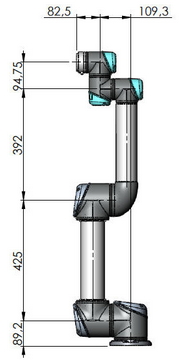
\includegraphics[scale=0.79]{Design/UR5measure.png}
    \caption{UR5 to describing DH-parameters \cite{DH}} 
    \label{fig:DH-Table} 
\end{figure}

%\begin{table}[h!]
%\centering
%\begin{tabular}{||c c c c c||} 
% \hline
% i & \alpha_{i-1} & a_{i-1} & d_{i} & \theta_{i} \\ [0.5ex] 
% \hline\hline
% 1 & 0 & 0  & 0     & \theta_{1} \\ 
% 2 & 0 & l_{1} & 0 & \theta_{2} \\
% 3 & 0 & l_{2} & 0 & \theta_{3} \\[1ex]
% \hline
%\end{tabular}
%\caption{DH-Table}
%\label{table:DH-table}
%\end{table}

As seen in \ref{fig:DH-Table},the coordinate systems is used to trace every step of each axis.\\
Starting from left to right at the top of the table, the $\alpha-1$ is used to compute the differences of the angles between $Z_{i}$ and $Z_{i-1}$, which is 0, due to the fact that they keep the same angle from $Z_{i}$  to $Z_{i-1}$.\\
It can also be seen from the table that the distance between $Z_{i}$ and $Z_{i-1}$ is Length2, since they are parallel to each other.\\ 
The distance between $X_{i-1}$ and $X_i$ is 0 since they cross each other on the perpendicular line, which means that in that point the new coordinate system should be placed.\\

\begin{table}[h!]
\centering
\begin{tabular}{||c c c c c||} 
 \hline
 i & \alpha_{i-1} & a_{i-1} & d_{i} & \theta_{i} \\ [0.5ex] 
 \hline 
 \hline
 1 & 0 & 0 & 89.2 & \theta_{1} \\ 
 2 & 90 & 0 & 0 & \theta_{2} \\
 3 & 0 & 425 & 0 & \theta_{3} \\
 4 & 0 & 392 & 109.3 & \theta_{4} \\
 5 & 90 & 0 & 94.75 & \theta_{5} \\ 
 6 & -90 & 0 & 82.5 & \theta_{6} \\[1ex] 
 \hline
\end{tabular}
\caption{DH-parameters for the UR5, using \cite{DHPar} as measurement.}
\label{table:1}
\end{table}

\section{Inverse Kinematics}
Inverse kinematics is used to compute the joint angles from a given position and orientation of an object\cite{JohnC}. The inverse kinematic can be set up from two aspects, one is the geometric way and the other is an algebraic solution, the one the team is using is the algebraic solution where the inverse kinematics is set up in MATLAB, a math computer program, where it makes it possible to be used later in computing the trajectory of the manipulator.\\
\section{Conclusion}

Describing a robot with forward kinematics and Denavit-Hartenberg parameters is used to locate the different joints and the tool in 3D-space, so the robot can be manipulated and used for various tasks.\\
Looking at Denavit-Hartenberg, the advantage of this method is to simplify the different axis in a matrix, so the operator and the robot can identify where the different coordinate systems is located.\\
Forward kinematics is the starting point of selecting the DH-parameters, when we know the point $Z_{1-1}$ and $Z_1$ we can then locate every axis in the desired robot. Hereby conclude to DH-parameters and include them into MATLAB while visualizing the robot and locate the robot so the tasks can be performed.\\
\chapter{Design}\label{Design}

\section{Desired Work-cell}

\begin{figure}[h]
    \centering
    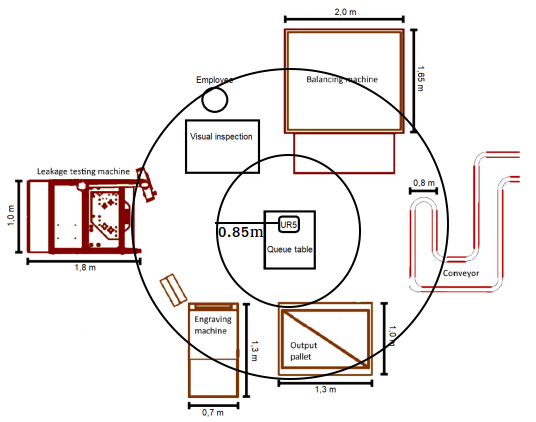
\includegraphics[width=9cm]{Design/Work_cell_3.png}
    \caption{work-cell with measurements and reach}
    \label{fig:workcellMR}
\end{figure}

When looking at \ref{fig:workcellMR}, a systematic work-cell is presented. But the important thing of a work-cell is its flow.\\
Here is some sections about what is needed of the ideal work-cell.

\subsection{Dexterous work-space}

The work-space which a manipulator works within can be described as a radius which the point of the end-effector can reach.\\
The Dexterous work-space is a more intelligent way of the robot to decide which points in arbitrary orientation, can be reached \cite{Dexterous}.\\
The reason that the dexterous work-space is considered a solution to the work-cell, is that the kinematic restrains can be included, so that the trajectories of the manipulator wont freeze or go in lock down.\\


\subsection{Safety}

To keep the production safe and manageable, some of the safety devices are chosen:

\begin{itemize}
    \item Light Curtain
    \item LIDAR
\end{itemize}

The light curtain provides a signal when the curtain is broken, see \ref{SafetyDevices}.\\
This will be used to send a signal to the UR5 to either stop or slow down the production, so a person safely can enter the cell, without getting serious damages.\\

The LIDAR is commonly used in production, see \ref{SafetyDevices}.
This threshold can be used to measure when a person enters the hazardous work area of the UR5.\\
All of the above is a must since the UR5 is carrying a metal rotor with sharp edges, so the person wont be gauged.\\

\subsection{Safety Requirements}

The most important solution for the safety of the work-cell, is the ISO 10218-2:2011, see \ref{ISO2}.\\
When installing a new robot for a production line, some standards is required. These standards of the ISO can present which of the areas needed to be acted upon.\\

\subsection{Placement Sensors}

To ensure the work-flow some intelligent placement sensors must be implemented. Some of the possible solutions are chosen:\\

\begin{itemize}
    \item LIDAR
    \item Photocell sensors
    \item Depth sensing camera
\end{itemize}

The LIDAR is a sensor that gives a 3D view, and can be used for the robot to tell the different object apart, and give an overview of the work-cell, see \ref{ref:PlacementS}.\\
These signals can be used for the cobot to get a better work-flow and also determine objects from each other.\\

The photocell sensors can be used for a quicker work-flow, since it will detect the rotors when they are in the correct place to be picked up, see \ref{ref:PlacementS}.\\

Depth sensing cameras can determine the distance from end-effector to the desired object, see \ref{ref:PlacementS}. This can be used to derive the distance from the certain machine where the rotor has to be placed.\\

\subsection{Conclusion}

When having looked into what an optimal layout for the work-cell could be, with regards to the above sections, it was concluded that it was also necessary to consider the robot manipulators that has to function within this space. 

\section{Desired Robot}\label{IdealRobot}

The ideal robot to have inside the work-cell, is intelligent, fast and can decide the next trajectory without any hesitation. Its size is optimized to fit the given case, to work at the most effective speed possible.\\

\subsection{Desired speed}

The robot has 7 tasks it needs to complete within 26 seconds. This means that the slowest possible speed it has to have per translation to other machines, while delivering the rotor, is 26 divided by 7, which will give the manipulator 3.7142 seconds to carry out the task.\\
Taking the visual inspection in consideration, the number has to be lower when translating from the machines. The person inspecting might need something close to 5 seconds. Taking that into consideration a new formula for the speed of the cobot can be found.\\

\begin{equation}
    26 = 5 + 6 \times b \Rightarrow b = \frac{21}{6}\\
\end{equation}

\begin{equation}
    b = \frac{21}{6} \Rightarrow b = \frac{7}{2}\\
\end{equation}

\begin{equation}
    b = \frac{7}{2} \Leftrightarrow  b = 3.5 sec\\
\end{equation}

5 seconds in one station means that the other stations needs to be cut down with 0.2 seconds each.\\
So the optimal speed for translations would be 3.5 seconds.\\

\subsection{Desired reach}

The manipulator must be able to reach all pick and place points, without having to move its base. Given the work-cell design, this means the robot will need a reach of 2 meters. \\
\begin{figure}[H]
    \centering
    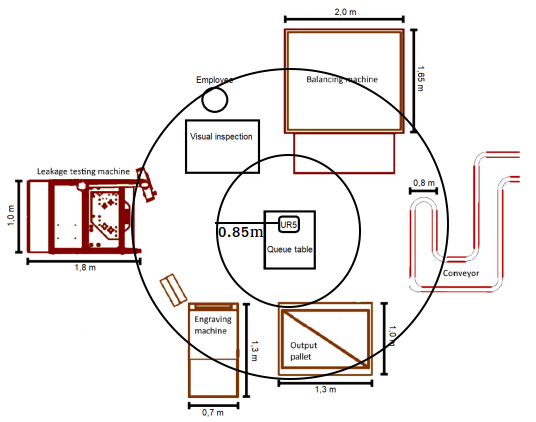
\includegraphics[width=8cm]{Design/Work_cell_3.png}
    \caption{Work-cell with measurements and reach}
    \label{fig:workcell}
\end{figure}

This desired reach could also be accomplished by changing the setup to use 2 manipulators, see figure \ref{fig:workscell2arms}. By doing it this way, the 2 robots would only need one place where their reach overlap, so they can both pick and place the rotors on a buffer table. This would also require additional programming, which should prevent the two robots from hitting each other.\\

\begin{figure}[H]
    \centering
    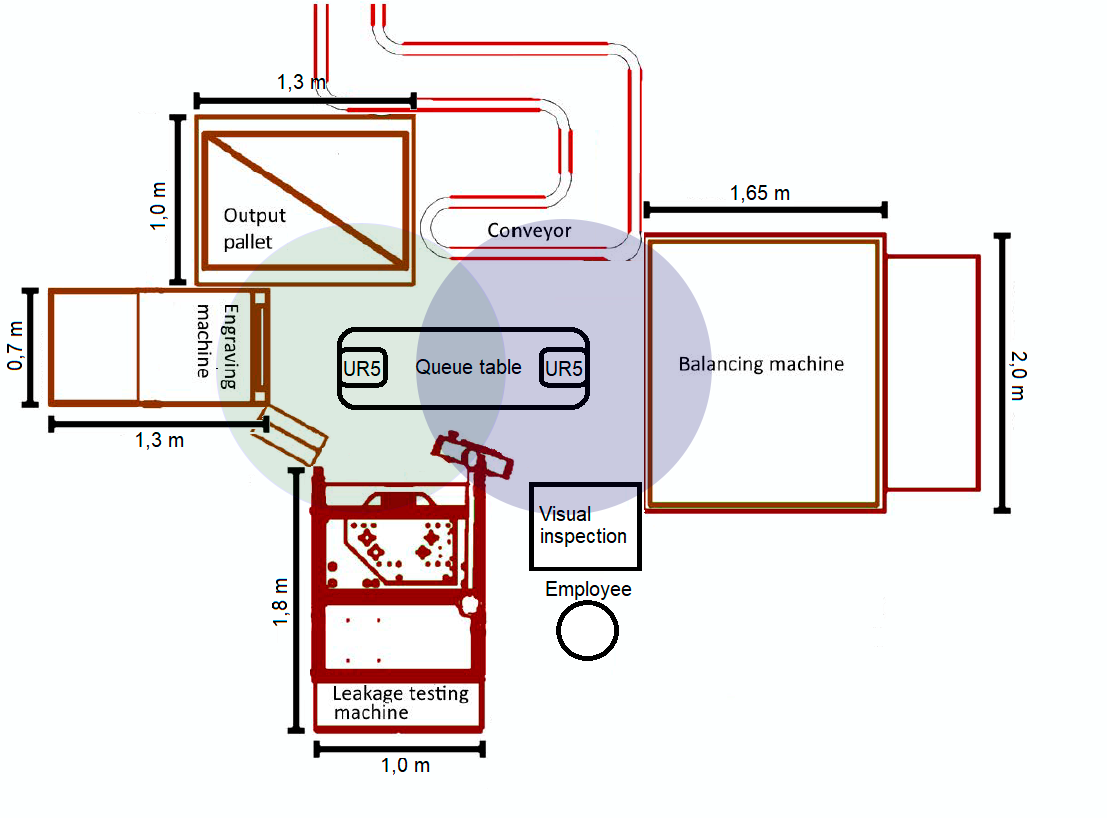
\includegraphics[width=.5\textwidth]{Design/Work_cell_8.PNG}
    \caption{Work-cell design with 2 robots}
    \label{fig:workscell2arms}
\end{figure}

\begin{figure}[H]
  \centering
  \begin{minipage}[b]{0.45\textwidth}
    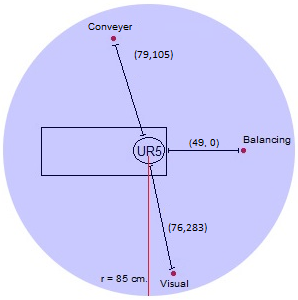
\includegraphics[width=\textwidth]{Design/workcell_1_polar.png}
    \label{fig:position}
  \end{minipage}
  \hfill
  \begin{minipage}[b]{0.45\textwidth}
    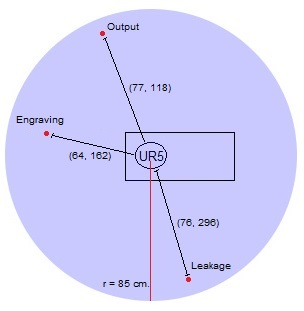
\includegraphics[width=\textwidth]{Design/polar.jpg}  
    \label{fig:velocity}
  \end{minipage}
  {Work-cell first and second part ,with polar coordinates and reach to suited the reach of the UR 5.}
\end{figure}
%Flowchart 1:
\begin{tikzpicture}[node distance=2cm]

%Primary nodes:
\node (start) [startstop] {Rotor arrives on conveyer/queue table};
\node (dec1) [decision, below of=start, yshift=-2.5cm] {Has this rotor been balance tested?};
\node (dec2) [decision, right of=dec1, xshift=3.2cm] {Is the balancing
machine empty?};
\node (pro1) [process, right of=dec2, xshift=3.1cm] {Move the rotor to balancing machine};
\node (out1) [io, below of=pro1, yshift=-3cm] {Balancing complete};
\node (dec3) [decision, below of=dec1, yshift=-6cm] {Has this rotor been visually inspected?};
\node (dec4) [decision, right of=dec3, xshift=3.2cm] {Is visual inspection available?};
\node (pro2) [process, right of=dec4, xshift=3.1cm] {Move the rotor to visual inspection};
\node (out2) [io, below of=pro2, yshift=-3cm] {Visual inspection complete};
\node (stop) [startstop, below of=dec3, yshift=-5cm] {Move rotor to queue table};

%Primary arrows:
\draw [arrow] (start) -- (dec1);
\draw [arrow] (dec1) -- node[anchor=south] {no} (dec2);
\draw [arrow] (dec1) -- node[anchor=west] {yes} (dec3);
\draw [arrow] (dec2) -- node[anchor=south] {yes} (pro1);
\draw [arrow] (pro1) -- (out1);
\draw [arrow] (dec3) -- node[anchor=south] {no} (dec4);
\draw [arrow] (dec3) -- node[anchor=west]  {yes} (stop);
\draw [arrow] (dec4) -- node[anchor=south] {yes} (pro2);
\draw [arrow] (pro2) -- (out2);

%dec2, dec4 -> start:
\node (gui1) [Guidebox, left of=pro1, xshift=-11cm] {};
\node (gui2) [Guidebox, below of=gui1, yshift=-0.85cm] {};
\node (gui6) [Guidebox, left of=pro2, xshift=-11cm] {};
\node (gui7) [Guidebox, below of=gui6, yshift=-0.85cm] {};

%Below dec2:
\node (gui3) [Guidebox, right of=gui2, xshift=5.9cm] {};
\node (gui4) [Guidebox, below of=gui3, yshift=1.9cm] {};
\node (gui5) [Guidebox, right of=gui3, xshift=-1.9cm] {};
\draw [arrow] (dec2) -- node[anchor=west] {no} (gui4);
\draw [arrow] (gui5) -- (gui2);

%Below dec4:
\node (gui8) [Guidebox, right of=gui7, xshift=5.9cm] {};
\node (gui9) [Guidebox, below of=gui8, yshift=1.9cm] {};
\node (gui10) [Guidebox, right of=gui8, xshift=-1.9cm] {};
\draw [arrow] (dec4) -- node[anchor=west] {no} (gui9);

%Line to start:
\node (gui11) [Guidebox, above of=gui1, yshift=2.55cm] {};
\node (gui12) [Guidebox, above of=gui11, yshift=-1.9cm] {};
\node (gui13) [Guidebox, left of=gui11, xshift=1.9cm] {};
\node (gui16) [Guidebox, below of=gui7, yshift=1.9cm] {};
\node (gui17) [Guidebox, left of=gui7, xshift=1.9cm] {};
\draw [arrow] (gui10) -- (gui17);
\draw [arrow] (gui16) -- (gui12);
\draw [arrow] (gui13) -- (start);

%out1, out2 -> dec3, stop:
\node (gui14) [Guidebox, above of=dec3, yshift=1cm] {};
\draw [arrow] (out1) -- (gui14);
\node (gui15) [Guidebox, above of=stop, yshift=-0cm] {};
\draw [arrow] (out2) -- (gui15);

%Caption:
\node (cap1) [Caption, below of=dec4, yshift=-7cm] {This flowchart shows the process performed by the first UR5 in the work-cell.};

\label{fig:first-part}
\end{tikzpicture}


%Flowchart 2:
\begin{tikzpicture}[node distance=2cm]

%Primary nodes:
\node (start) [startstop] {Rotor arrives on queue-table};
\node (dec1) [decision, below of=start, yshift=-2.5cm] {Has this rotor been leak tested?};
\node (dec2) [decision, right of=dec1, xshift=3.2cm] {Is the leak testing
machine empty?};
\node (pro1) [process, right of=dec2, xshift=3.1cm] {Move the rotor to leak testing machine};
\node (out1) [io, below of=pro1, yshift=-3cm] {Leak testing complete};
\node (dec3) [decision, below of=dec1, yshift=-6cm] {Has this rotor been engraved?};
\node (dec4) [decision, right of=dec3, xshift=3.2cm] {Is the engraving
machine empty?};
\node (pro2) [process, right of=dec4, xshift=3.1cm] {Move the rotor to engraving machine};
\node (out2) [io, below of=pro2, yshift=-3cm] {Engraving complete};
\node (stop) [startstop, below of=dec3, yshift=-5cm] {Move rotor to output pallet};

%Primary arrows:
\draw [arrow] (start) -- (dec1);
\draw [arrow] (dec1) -- node[anchor=south] {no} (dec2);
\draw [arrow] (dec1) -- node[anchor=west] {yes} (dec3);
\draw [arrow] (dec2) -- node[anchor=south] {yes} (pro1);
\draw [arrow] (pro1) -- (out1);
\draw [arrow] (dec3) -- node[anchor=south] {no} (dec4);
\draw [arrow] (dec3) -- node[anchor=west]  {yes} (stop);
\draw [arrow] (dec4) -- node[anchor=south] {yes} (pro2);
\draw [arrow] (pro2) -- (out2);

%dec2, dec4 -> start:
\node (gui1) [Guidebox, left of=pro1, xshift=-11cm] {};
\node (gui2) [Guidebox, below of=gui1, yshift=-0.85cm] {};
\node (gui6) [Guidebox, left of=pro2, xshift=-11cm] {};
\node (gui7) [Guidebox, below of=gui6, yshift=-0.85cm] {};

%Below dec2:
\node (gui3) [Guidebox, right of=gui2, xshift=5.9cm] {};
\node (gui4) [Guidebox, below of=gui3, yshift=1.9cm] {};
\node (gui5) [Guidebox, right of=gui3, xshift=-1.9cm] {};
\draw [arrow] (dec2) -- node[anchor=west] {no} (gui4);
\draw [arrow] (gui5) -- (gui2);

%Below dec4:
\node (gui8) [Guidebox, right of=gui7, xshift=5.9cm] {};
\node (gui9) [Guidebox, below of=gui8, yshift=1.9cm] {};
\node (gui10) [Guidebox, right of=gui8, xshift=-1.9cm] {};
\draw [arrow] (dec4) -- node[anchor=west] {no} (gui9);

%Line to start:
\node (gui11) [Guidebox, above of=gui1, yshift=2.55cm] {};
\node (gui12) [Guidebox, above of=gui11, yshift=-1.9cm] {};
\node (gui13) [Guidebox, left of=gui11, xshift=1.9cm] {};
\node (gui16) [Guidebox, below of=gui7, yshift=1.9cm] {};
\node (gui17) [Guidebox, left of=gui7, xshift=1.9cm] {};
\draw [arrow] (gui10) -- (gui17);
\draw [arrow] (gui16) -- (gui12);
\draw [arrow] (gui13) -- (start);

%out1, out2 -> dec3, stop:
\node (gui14) [Guidebox, above of=dec3, yshift=1cm] {};
\draw [arrow] (out1) -- (gui14);
\node (gui15) [Guidebox, above of=stop, yshift=-0cm] {};
\draw [arrow] (out2) -- (gui15);

%Caption:
\node (cap1) [Caption, below of=dec4, yshift=-7cm] {This flowchart shows the process performed by the second UR5 in the work-cell.};

\end{tikzpicture}






\subsection{Desired sensors}

The robot should be able to identify humans, and collisions must be risk free, and not disrupt the work-flow. Optimally, the robot should also be able to identify what object it is holding, and if it is damaged or not. Additionally, the robot must be able to place the rotors correctly in the machines, using a depth sensing camera. \ref{depthcam}\\
The robot should be able to register whether or not it has picked up a rotor. This can be done by using a pressure sensor.\\ 

\subsection{Max payload}
The robot manipulator must be able to lift the combined weight of the L40 rotor, aswell as the end-effector tool meant to lift and move the rotor. For this reason, the combined weight of the end-effector tool and the L40 rotor can not exceed a total weight of 5 Kg.\\

%\ref{workscell2arms}. this ref is not linking to anything??
%The robot must be able to lift the L40 rotor given in the case, which weighs 645 grams. The end-effector must also be able to grab it, without the risk of dropping it. The rotor is 190mm long, and 90mm wide at its widest point. The manipulator must also be able to support the[width=8cm] weight when the arm is fully stretc\ref{workscell2arms}

\subsection{Conclusion}

From this chapter several specifications can be derived, which is required to setup a robot manipulator, these data and considerations will thus be used for the next section, which will describe these requirements.


\section{Denavit-Hartenberg}

In order to enable the UR5 on the flexible workstation to locate itself and its surroundings within a space, the DH (Denavit-Hartenberg) method is used.\\ 
The DH method can be used to compute every frame into parameters.\\
These descriptions of the system can be used to translate every point and every movement of the robotic manipulator, with the help of forward kinematic.\\
Initially the start is to locate all of the coordinate systems, as seen in \ref{table:1}.\\ 


\begin{itemize}
    \item ${a_{i-1}}$= The distance from ${Z_{i-1}}$ to ${Z_{i}}$ measured along ${X_{i-1}}$
    \item ${\alpha_{i-1}}$ = The angel between ${Z_{i-1}}$ to ${Z_{i}}$ measured about ${X_{i-1}}$
    \item ${d_{i}}$ = The distance from ${X_{i-1}}$ to ${X_{i}}$ measured along ${Z_{i}}$
    \item ${\theta_{i-1}}$ = The angel between ${X_{i-1}}$ to ${X_{i}}$ measured about ${Z_{i}}$
\end{itemize}



Then the angles and the distance from each coordinate system is computed and set in to a table as seen in \ref{fig:DH-Table}.

\begin{figure}[h!]
    \centering
    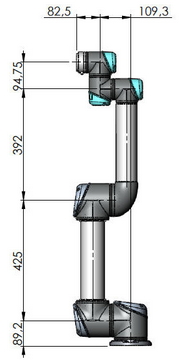
\includegraphics[scale=0.79]{Design/UR5measure.png}
    \caption{UR5 to describing DH-parameters \cite{DH}} 
    \label{fig:DH-Table} 
\end{figure}

%\begin{table}[h!]
%\centering
%\begin{tabular}{||c c c c c||} 
% \hline
% i & \alpha_{i-1} & a_{i-1} & d_{i} & \theta_{i} \\ [0.5ex] 
% \hline\hline
% 1 & 0 & 0  & 0     & \theta_{1} \\ 
% 2 & 0 & l_{1} & 0 & \theta_{2} \\
% 3 & 0 & l_{2} & 0 & \theta_{3} \\[1ex]
% \hline
%\end{tabular}
%\caption{DH-Table}
%\label{table:DH-table}
%\end{table}

As seen in \ref{fig:DH-Table},the coordinate systems is used to trace every step of each axis.\\
Starting from left to right at the top of the table, the $\alpha-1$ is used to compute the differences of the angles between $Z_{i}$ and $Z_{i-1}$, which is 0, due to the fact that they keep the same angle from $Z_{i}$  to $Z_{i-1}$.\\
It can also be seen from the table that the distance between $Z_{i}$ and $Z_{i-1}$ is Length2, since they are parallel to each other.\\ 
The distance between $X_{i-1}$ and $X_i$ is 0 since they cross each other on the perpendicular line, which means that in that point the new coordinate system should be placed.\\

\begin{table}[h!]
\centering
\begin{tabular}{||c c c c c||} 
 \hline
 i & $\alpha_{i-1}$ & $a_{i-1}$ & $d_{i}$ & $\theta_{i}$ \\ [0.5ex] 
 \hline 
 \hline
 1 & 0 & 0 & 89.2 & $\theta_{1}$ \\ 
 2 & 90 & 0 & 0 & $\theta_{2}$ \\
 3 & 0 & 425 & 0 & $\theta_{3}$ \\
 4 & 0 & 392 & 109.3 & $\theta_{4}$ \\
 5 & -90 & 0 & 94.75 & $\theta_{5}$ \\ 
 6 & 90 & 0 & 82.5 & $\theta_{6}$ \\[1ex] 
 \hline
\end{tabular}
\caption{DH-parameters for the UR5, using \cite{DHPar} as measurement.}
\label{table:1}
\end{table}

\section{Forward Kinematics}
Forward kinematics can be used for calculating the position and orientation of the end-effector of a robotic manipulator. This can be done by using the matrices describing the position and orientation of each of the joints for the specific robotic manipulator, and the following formula: \\

\begin{equation}
    _N^0 T\; =\ _1^0T\  _2^1T\  _3^2T\  _4^3T\  .........\  _N^{N-1}T\\
\end{equation} \\

This is the formula used for calculating the end-effector of a robotic manipulator. \\

Now, the required transformation matrices can simply be inserted into the formula, and the matrix describing the position of the end-effector can be calculated. \\

Below are the general transformation matrices used in this method; from the base of the robotic manipulator to the sixth joint. These can be multiplied together to find \(_6^BT\) for the UR5: 

\begin{equation}
\centering
_i^{i-1}T = \begin{bmatrix} Cos(\theta_i) & -Sin(\theta_i) & 0 & a_{i-1}\\
Sin(\theta_i)*Cos(\alpha_{i-1}) & Cos(\theta_i)*Cos(\alpha_{i-1}) & -Sin(\alpha_{i-1}) & -Sin(\alpha_{i-1})*d_i\\
Sin(\theta_i)*Sin(\alpha_{i-1})& Cos(\theta_i)*Sin(\alpha_{i-1}) & Cos(\alpha_{i-1}) & Cos(\alpha_{i-1})*d_i \\
0 & 0 & 0 & 1\\ \end{bmatrix}
    \caption{Caption}
    \label{fig:my_label}
\end{equation}
\\


\begin{equation}
\centering
_0^BT = \begin{bmatrix} 1&0&0&0\\0&1&0&0\\0&0&1&0\\ 0&0&0&1\end{bmatrix}
    \caption{Caption}
    \label{fig:tb0}
\end{equation}

\begin{equation}
\centering
_1^0T = \begin{bmatrix} Cos(\theta_1)&-Sin(\theta_1)&0&0\\Sin(\theta_1) & Cos(\theta_1)&0&0\\0&0&1& d_1\\0&0&0&1 \end{bmatrix}
    \caption{Caption}
    \label{fig:t01}
\end{equation}

\begin{equation}
\centering
_2^1T = \begin{bmatrix} Cos(\theta_2)&-Sin(\theta_2)&0&0\\
0&0&-1&0\\Sin(\theta_2)& Cos(\theta_2)&0&0\\0&0&0&1\end{bmatrix}
    \caption{Caption}
    \label{fig:t12}
\end{equation}

\begin{equation}
\centering
_3^2T = \begin{bmatrix} Cos(\theta_3)&-Sin(\theta_3)&0&a_2\\
Sin(\theta_3)&Cos(\theta_3)&0&0\\0&0&1&0\\0&0&0&1\end{bmatrix}
    \caption{Caption}
    \label{fig:t23}
\end{equation}
\begin{equation}
\centering
_4^3T = \begin{bmatrix} Cos(\theta__4)&-Sin(\theta_4)&0&a__3\\
Sin(\theta_4)&Cos(\theta_4)&0&0\\0&0&1& d_4\\0&0&0&1\end{bmatrix}
    \caption{Caption}
    \label{fig:t34}
\end{equation}

\begin{equation}
\centering
_5^4T = \begin{bmatrix} Cos(\theta_5)&-Sin(\theta_5)&0&0\\
0&0&1&d_5\\-Sin(\theta_5)&-Cos(\theta_5)&0&0\\0&0&0&1\end{bmatrix}
    \caption{Caption}
    \label{fig:t45}
\end{equation}

\begin{equation}
\centering
_6^5T = \begin{bmatrix} Cos(\theta_6)&-Sin(\theta_6)&0&0\\https://www.sharelatex.com/project/5a829b040d7aa54a74a65ba0
0&0&-1&-d_6\\Sin(\theta_6)&Cos(\theta_6)&0&0\\0&0&0&1\end{bmatrix}
    \caption{Caption}
    \label{fig:t56}
\end{equation}

 \\\


The main idea is, given the joint angles as input, you would be able to get the coordinates for the end-effector as output. So the position can be calculated from specific set values, and used for simulations.\\

Kinematics can be used to form an internal picture in a cartesian space  of the robot movements, and help understanding and explaining it. 

This is useful when working with not only manipulators, but also animations in movies and video games, or any other movement where multiple joints are used. 



\section{Inverse Kinematics}
Inverse kinematics is used to compute the joint angles from a given position and orientation of an object\cite{JohnC}. The inverse kinematic can be set up from two aspects, one is the geometric way and the other is an algebraic solution, the one the team is using is the algebraic solution where the inverse kinematics is set up in MATLAB, a math computer program, where it makes it possible to be used later in computing the trajectory of the manipulator.\\




\section{Conclusion} 

Describing a robot with forward kinematics and Denavit-Hartenberg parameters is used to locate the different joints and the tool in 3D-space, so the robot can be manipulated and used for various tasks.\\
Looking at Denavit-Hartenberg, the advantage of this method is to simplify the different axis in a matrix, so the operator and the robot can identify where the different coordinate systems is located.\\
Forward kinematics is the starting point of selecting the DH-parameters, when we know the point $Z_{1-1}$ and $Z_1$ we can then locate every axis in the desired robot. Hereby conclude to DH-parameters and include them into MATLAB while visualizing the robot and locate the robot so the tasks can be performed.\\












\chapter{Requirements specification} \label{ch:IdealReq}

%\begin{itemize}
%    \item A rotor cycle time may not exceed, 26 second within the work-cell.
%    \item The cycle within the work-cell must be ergonomic for the co-worker and reduce work-stress.
%    \item An emergency stop must always be in reach of an operator
%    \item The safety of the work-cell must comply with the ISO standards 10218-2:2011.
%    \item The manipulator must provide a better work-flow than a human alone.
%    \item Each machine must be within reach of at least one of the robotic manipulators.
%    \item The manipulator must be able to lift a payload of 645g at maximum reach.
%    \item The manipulator must be signaled by the sensors in the machines, to handle different tasks.
%    \item The setup must be flexible to accommodate for new machines within.
%\end{itemize}
\section{Delimitations} \label{ch:Delimitations}

The requirements for the desired robot is not what is available for the project. 
The work-cell that is given to the group by AAU, is not nearly big enough to cover the desired reach of the manipulator. As the case describes, see \ref{fig:workcellMR}, the reach of the manipulator has to be the same as 2 meters. The desired work-cell can simply not be downsized to a shorter distance, without having to close the work-cell completely from entry.\\
To delimit the reach, a new solution had to be made, which is why the group decided to implement another manipulator on the opposite side of the Queue-table. This has to be delimited as well since the group do not have permission or knowledge to implement 2 UR5's on the same table.\\
%For testing purposes, the work-cell can be simulated in a 2:1 scale, requiring half the space, and making the tests possible. \\
The required speed for the manipulator can in theory be done since the manipulator assigned to the group has a speed of 1m/s. The only delimitation is that, if the group want to get this speed, a default setting on the UR5 has to be overridden. so that it will be able to move at maximum velocity \cite{UserManual}.\\.
%Looking at the sensors, the only available sensor for the group is in the UR5, which is the pressure sensor. This is a delimitation for the safety process of this project. However, the sensors can be simulated with another method, for example a command that can be implemented in the code of the UR5.\\

\newpage
\section{Delimited requirement specifications}

\begin{enumerate}
    \item The cycle time of the rotor must not exceed 26 seconds.
    \item It is required that the cobot differentiates the height of the rotor for visual inspection every hour. so the visual inspector is forced to not stay in the static position throughout the entire workday.
    \item The emergency stops has to stop the entire work-cell.
    \item The work-cell must have at least one emergency stop placed, so the worker can reach the stops without putting himself to harm.
    \item The UR5 must be able to have a lifting capacity more than the total combined payload of the rotor(645g) and the end-effector(500g) at maximum reach.
    \item The UR5 must perform this task when signalled by the placement sensor in:\\
    1. Balancing machine: Put the rotor in the control-box, if the placement sensor has signalled that the prior rotor has been removed.\\
    2. Leak testing machine: Put both rotors in the leak-test, make sure only to remove them when the two rotors has been tested. Ensure that the rotor has been balanced before inserting.\\
    3. Engraving machine : The rotors orientation must be upside-down, while placing the rotor. Also ensure that the rotor that is picked has been in the 2 prior machines.
    \item When a worker enters the work-cell, the velocity of the end-effector on the UR5 has to slow down to 0,1 m/s, to reduce the risk of harmful behaviour.\\
    \item The rotor has to be placed whit in a radius of 1mm of a specific position. 
    \end{enumerate}


\section{Delimitation's} \label{ch:Delimitations}

The requirements for the ideal robot is not what is available for the project. 
The work-cell that is given to the group by AAU, is not nearly big enough to cover the desired reach of the manipulator. As the case describes, see \ref{fig:workcellMR}, the reach of the manipulator has to be the same as 2 meters. The ideal work-cell can simply not be cut down to a shorter distance, without having to close the work-cell completely from entry.\\
Delimiting the reach, a new solution had to be made, which is why the group decided to implement another manipulator on each side of the pallet-table. This has to be delimited as well since the group doesn't have permission or knowledge to implement 2 UR5's on the same table.
For testing purposes, the work-cell can be simulated in a 2-1 scale, requiring half the space, and making the tests possible. \\
The required speed for the manipulator can in theory be done since the manipulator assigned to the group has a speed of 1m/s. The only delimitation is that, if you want to get this speed, a default setting on the UR5 has to be overridden, so that it will move with maximum speed \cite{UserManual}.\\
Also the machinery have some time-consuming processes, hereby the threshold of 26 seconds might be exceeded.\\
Looking at the sensors, the only available sensor for the group is in the UR5, which is the pressure sensor. This is a delimitation for the safety process of this project. However the sensors can be simulated with another method, for example a command that can be implemented in the code of the UR5.\\

\section{Final Problem formulation} \label{ch:finalprob}
 %How can the manipulator be set up to safely cooperate with humans within a work-cell, while the manipulator upholds the specified work-flow  time-limit of a rotor-cycle and the required specifications. 
 %How can the manipulator be set up to comply with the required specifications of not exceeding the 26 second cycle limit, while taking into consideration of the safety and ergonomic relations to the co-workers around it, in a flexible way to be able to accommodate changes to the work-cell.
 
 
 How is it possible for the UR5 to pick and place the rotors in the desired orientation and location of the work-cell, while upholding the cycle limit of 26 seconds and safety requirements of the work-cell? 
 
 
 
\chapter{UR5 - Delimited Cobot}

In this chapter the specifications of the delimited cobot will be presented.

\section{UR}

Universal Robots was founded in 2005 by a group of Danish engineers. Their thought was, that every industrial robot on the market was designed to be big, heavy and expensive. Therefore the group decided to make a smaller and more agile kind of industrial robot.\cite{Urhist}\\
Here are the specification for the UR5:\\ 

\subsubsection{UR5}

\begin{itemize}
    \item Weight: 18.4 kg.
    \item Payload: 5 kg.
    \item Footprint: 149 mm.
    \item Joints: +/-360 degrees on all the joints.
    \item Operating life: 35,000 Hours.
    \item Speed: joints = 180 degrees/sec, tool = 1 m/sec.
    \item Reach: 850 mm.
    \item Repeatability: +/- 0.1 mm.
\end{itemize}

The materials used on all the cobots are aluminum and plastic\cite{Ur5_about}\cite{UR5_tech}.\\

\begin{figure}
    \centering
    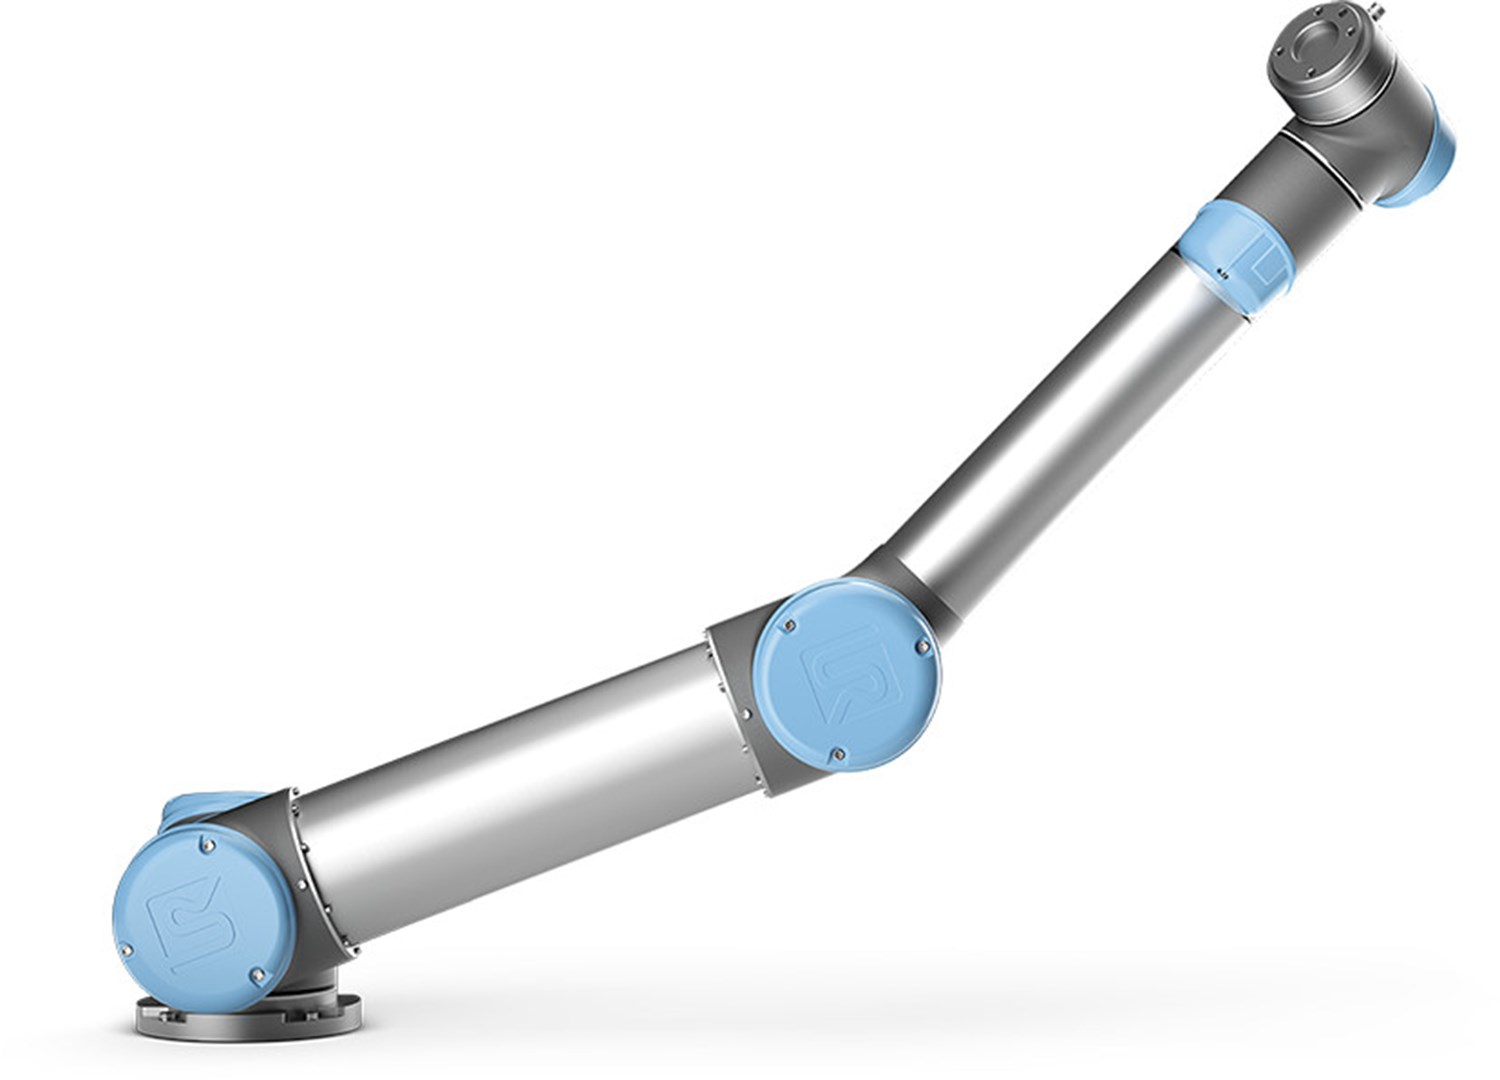
\includegraphics[width=9cm]{UR/UR5pic.jpg}
    \caption{Universal Robots UR5 \cite{UR5billede}}
    \label{fig:UR5}
\end{figure}

Looking in to the specifications of the UR5 some delimited requirements can be written:\\
 



\section{Delimited requirement specifications}

\begin{itemize}
    \item A rotor cycle may not exceed 26 seconds within the work-cell
    \item The cycle of the rotor inside the work-cell must be ergonomic.
    \item The emergency stop must always be in reach of an operator.
    \item The UR5 must operate the rotor faster than a human.
    \item At least 4 points (Machines) in the work-cell must be within reach of the UR5.
    \item The UR5 must be able to lift a payload of 645g in 0 posistion.
    \item The UR5's programming must be flexible, so it wont lower the production time when a new machine is presented.
    \item The UR5 must react to the different tasks given to it by sensors.
\end{itemize}
%%begin novalidate
%backmatter
\appendix
\listoftodos
\printbibliography[heading=bibintoc]
%\printbibliography[heading=]
%\bibliographystyle{IEEEtrans}
%\bibliography{references}
\label{bib:mybiblio}
\titleformat{%command
  \chapter
}[%shape
display%
]{%format
  \normalfont\huge
}{%label
  \begin{center}\color{aaublue}\chaptertitlename\ \thechapter\end{center}
}{%style
  1cm
}{%code before title
  \thispagestyle{empty}\begin{center}\Large
}[%code after title
  \end{center}
]
%%end novalidate

\end{document}
